\documentclass[resume]{subfiles}


\begin{document}
\section{Kalman}
C'est un algorithme de \textbf{data fusion} utilisé pour
\begin{itemize}
\item Filtre des données bruitées
\item Estimer l'état d'un système
\end{itemize}
Le système est donné par
$$\boxed{x_t=Ax_{t-1}+Bu_{t}+\textcolor{Violet}{w_t}}$$
Avec $\textcolor{Violet}{w_t}$ le bruit de process. Si on souhaite mesurer le système il existe également un bruit de mesure $\textcolor{Violet}{v_t}$. Les deux bruits sont des bruits blancs gaussiens.
$$z_t=Hx_t+\textcolor{Violet}{v_t}$$
\subsection{Propriétés}
Si
\begin{itemize}
\item Le système est "bien modélisé"
\item Le système est linéaire et mono dimensionnel
\item Les bruits de mesure sont WGN
\end{itemize}
Alors le filtre de Kalman a été prouvé être l'estimateur optimal
\subsection{Fonctionnement}
\begin{enumerate}
\item Prédiction
\item Correction (amélioration de l'estimation)
\end{enumerate}
\subsubsection{Prédiction}
$$\hat{x}_{t|t-1}=A\hat{x}_{t-1|t-1}+Bu_t$$
$$P_{t|t-1}=AP_{t-1|t-1}A^{T}+Q_t$$
Mise à jour de la matrice de covariance $P$
$$P_{t|t-1}=AP_{t-1|t-1}A^T+Q_t$$
\subsubsection{Correction}
$$\hat{x}_{t|t}=\hat{x}_{t|t-1}+K_t(y_t-H\hat{x}_{t|t-1})$$
$$P_{t|t}=P_{t|t-1}-K_tH_tP_{t|t-1}$$
Avec $K_t$ la matrice de gain de Kalman
$$K_t=P_{t|t-1}H_t^T(H_tP_{t|t-1}H-t^T+R_t)^{-1}$$
\subsubsection{Fusions de deux densités de probabilité}
$$y_1=\frac{1}{\sqrt{2\pi \sigma_1^2}}e^{-\frac{(r-\mu_1)^2}{2\sigma_1^2}}$$
$$y_2=\frac{1}{\sqrt{2\pi \sigma_2^2}}e^{-\frac{(r-\mu_2)^2}{2\sigma_2^2}}$$
$$y_{1+2}=\frac{1}{2\pi\sigma_1\sigma_2}e^{-\left(\frac{(r-\mu_1)^2}{2\sigma_1^2}+\frac{(r-\mu_2)^2}{2\sigma_2^2}\right)}$$
$$\boxed{\mu_{12}=\mu_1+\frac{\sigma_1^2}{\sigma_1^2+\sigma_2^2}\left(\mu_2-\mu_1\right)}$$
$$\boxed{\sigma_{12}^2=\sigma_1^2-\frac{\sigma_1^4}{\sigma_1^2+\sigma_2^2}}$$
Il faut faire attention à tout ramener au même domaine avant de rassembler les mesures.
\subsubsection{Matrices $H$ et $K$}
$$H=\frac{1}{c}$$
$$K=\frac{H\sigma_1^2}{H^2\sigma_1^2+\sigma_2^2}$$
$$\mu_{12}=\mu_1+K(\mu_2-H\mu_1)$$
$$\sigma_{12}^2=\sigma_1^2-KH\sigma_1^2$$
\subsubsection{Équations de récurrence}
$$\hat{x}_{t|t}=\hat{x}_{t|t-1}+K_t(z_t-H_t\hat{x}_{t|t-1})$$
$$P_{t|t}=P_{t|t-1}-K_tH_tP_{t|t-1}$$
\begin{figure}[H]
\centering
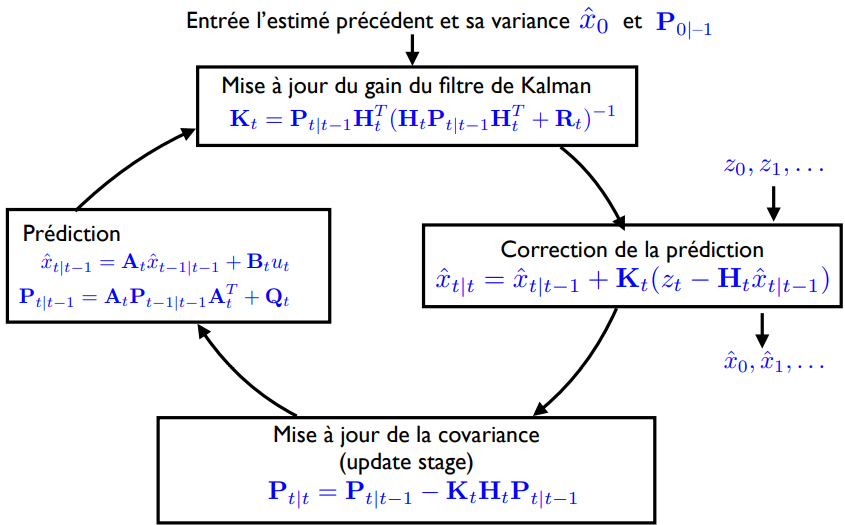
\includegraphics[width=\columnwidth]{img_22.png}
\end{figure}








\subsubsection{Matrice de covariance}
$$P_t=\begin{bmatrix}
\text{Var}(x_t^{1}) & \text{Covar}(x_t^{1}x_t^{2}) & \cdots & \text{Covar}(x_t^{1}x_t^{n})\\
\text{Covar}(x_t^{2}x_t^{1}) & \text{Var}(x_t^{2}x_t^{2}) & \cdots & \vdots\\
\vdots & \vdots & \ddots & \vdots\\
\text{Covar}(x_t^{n}x_t^{1}) & \text{Covar}(x_t^{n}x_t^{2}) & \cdots & \text{Var}(x_t^{n})
\end{bmatrix}$$
\subsection{Linéarisation}
Si le système est non-linéaire, tout s'écroule. Il convient alors de linéariser le système.
$$x_{k+1}\approx f(\bar{x}_k,u_k)+\frac{\del f}{\del x}(\bar{x}_k,u_k)\Delta x_k+w_k$$
$$y_k\approx g(\bar{x}_k)+\frac{\del g}{\del x}(\bar{x}_k,u_k)\Delta x_k+v_k$$
Voir page 32







\end{document}